\section{Stars and Galaxies}
\subsection{The Life Cycle of Stars}
Stars are massive celestial objects primarily composed of hydrogen and helium. They generate energy through \textbf{nuclear fusion}. The evolution of a star depends largely on its \textit{initial mass}.

The Sun has a mass of approximately \qty{1.989e30}{\kilogram}. Its effective surface temperature is about \qty{5772}{\kelvin}.

The mass--energy equivalence is expressed as:
\begin{equation}
    E = mc^2
    \label{eq:mass-energy}
\end{equation}

\textcite{carroll2007} describe stellar structure and evolution in detail. Selected properties of stars are summarized in Table~\ref{tab:stellar-properties}.

\begin{table}[htbp]
    \centering
    \caption{Illustrative properties of selected stars}
    \label{tab:stellar-properties}
    \begin{tabular}{lcr}
        \toprule
        Star & Type & Mass ($M_\odot$) \\
        \midrule
        Sun & G-type & 1.0 \\
        Sirius A & A-type & 2.1 \\
        Betelgeuse & Red supergiant & 16.5 \\
        \bottomrule
    \end{tabular}
\end{table}

\subsection{Types of Galaxies}
Galaxies can be classified into several major categories:
\begin{itemize}
    \item Spiral galaxies
    \item Elliptical galaxies
    \item Irregular galaxies
\end{itemize}

\begin{figure}[htbp]
    \centering
    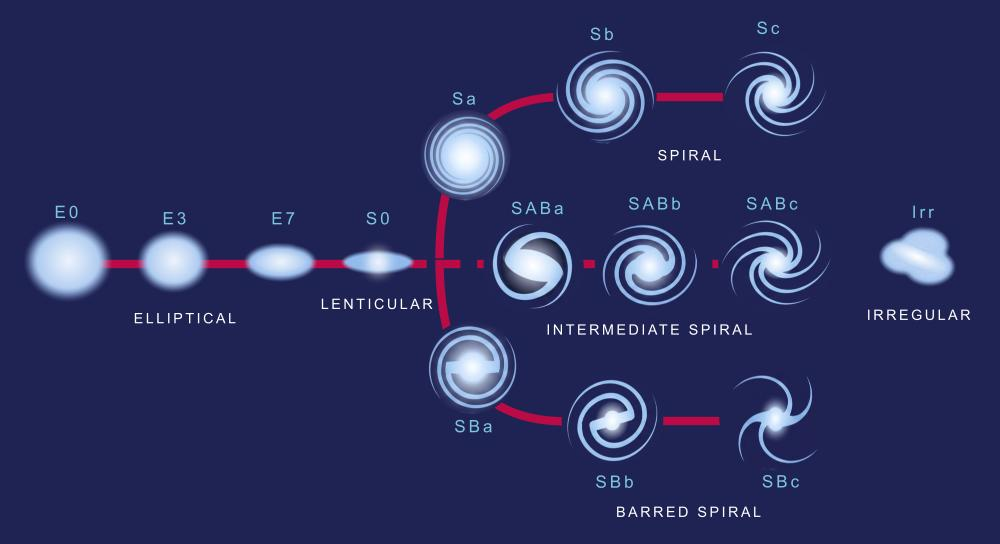
\includegraphics[width=0.8\textwidth]{figures/images/galaxy-types.jpg}
    \caption{Major galaxy morphologies: spiral, elliptical, and irregular.}
    \label{fig:galaxy-types}
\end{figure}

The main morphological categories are summarized in Table~\ref{tab:galaxy-types}.
\begin{table}[htbp]
    \centering
    \caption{Basic galaxy classifications}
    \label{tab:galaxy-types}
    \begin{tabular}{ll}
        \toprule
        Galaxy type & Typical characteristic \\
        \midrule
        Spiral & Disk with spiral arms \\
        Elliptical & Smooth, rounded appearance \\
        Irregular & No regular overall shape \\
        \bottomrule
    \end{tabular}
\end{table}